% ============================================================================ 4 · Datos técnicos relevantes
\section{Datos técnicos relevantes}
\label{sec:datos}

Esta sección es la respuesta al criterio de \emph{calidad del tratamiento de datos}. Contamos qué llegó, qué
trampas tenía, qué descartamos y por qué, y cómo quedó trazado cada paso. Las dificultades son parte del
resultado: varias cosas que creíamos saber con la primera entrega dejaron de ser ciertas con la segunda.

\subsection{Las tres tablas: lo que prometía el anexo y lo que llegó}

Ford describe tres tablas (anexo 7 del desafío): \emph{Trip Summary} (estado del vehículo al inicio y al
final de cada viaje), \emph{DynamicInformation} (estados en cada envío de datos) y \emph{Vehicle General
Information} (datos estáticos). Llegaron como seis CSV, cada tabla partida en dos cohortes de muestreo:
vehículos con evento registrado (\emph{Failed}) y sin evento (\emph{NotFailed}).

\begin{table}[H]
\centering
\caption{Los archivos de las dos entregas. La telemetría de los sanos de la entrega v2 es byte a byte la de
la entrega 1: todo lo nuevo está en la estática y en los archivos de fallados.}
\label{tab:archivos}
\small
\begin{tabular}{@{}llrrl@{}}
\toprule
Tabla & Cohorte & Filas, entrega 1 (15-09) & Filas, entrega v2 (26-09) & ¿Igual? \\
\midrule
Estática & fallados & 378 & 298 & no \\
Estática & sanos & 742 & 768 & no \\
Viajes (\emph{TripSummary}) & fallados & 947.477 & 934.463 & no \\
Viajes (\emph{TripSummary}) & sanos & 1.583.958 & 1.583.958 & sí \\
Señales (\emph{DynamicInformation}) & fallados & 4.202.484 & 3.595.216 & no \\
Señales (\emph{DynamicInformation}) & sanos & 6.415.333 & 6.415.333 & sí \\
\bottomrule
\end{tabular}
\fuente{\repo{docs/\allowbreak{}memoria/\allowbreak{}f9-entrega-v2.md} §1 y \repo{f1-datos-reales.md}; reproduce
\repo{scripts/\allowbreak{}compare\_deliveries.py}.}
\end{table}

\textbf{Qué encontramos al contrastar contra el anexo} (detalle en el Anexo~\ref{anx:tablas}):
\begin{itemize}
  \item \textbf{\emph{TripSummary} trae 25 de las 40 columnas documentadas.} Faltan 19: GPS (4), elevación (2),
    presión de neumáticos (8), hollín de regeneración manual (2), autonomía (1) y el DPF por su nombre (2).
    Aparecen 4 que el anexo no menciona: \texttt{AirFilterStart/\allowbreak{}End} y \texttt{AirRegenerationStart/\allowbreak{}End}, que
    son el DPF con otro nombre (§\ref{sec:desafio}).
  \item \textbf{\emph{DynamicInformation} y la estática cierran} (7 y 7 columnas), con renombres cosméticos:
    \texttt{Vin} → \texttt{VehicleCode}, \texttt{SalesCountryCd} → \texttt{SalesCountry\_cd}. No hay VIN: el
    único identificador es \texttt{VehicleCode}, y el join entre las tres tablas cierra.
  \item \textbf{El evento no está marcado fila a fila}: sale del vehículo. \texttt{IdentificationDate} está en
    el 100\,\% de los fallados y es nula en el 100\,\% de los sanos. \textbf{La cohorte es la etiqueta}, y por
    eso nunca entra como variable.
  \item \textbf{\texttt{Regenerations} no es un booleano}: es el texto literal \texttt{“Regeneration”} que marca
    una fila. Declararla numérica la convertía en nula en silencio.
  \item Los seis archivos vienen con BOM: si no se leen como \texttt{utf-8-sig}, la primera
    columna sale con el BOM pegado al nombre y el join falla.
\end{itemize}

\subsection{Equipos o sistemas existentes: el histórico por vehículo}

\textbf{Qué entendimos.} El documento promete un histórico de recolección por vehículo, con autos con y sin
degradación, y deja la periodicidad y el volumen a confirmar.

\textbf{Qué encontramos.} Hay historial de sobra para ventanas de varios miles de km. Con la primera
entrega, la mediana por vehículo era de \textasciitilde2.000 viajes, \textasciitilde7.000–8.000 señales,
\textasciitilde17.000–21.000 km de odómetro final y 400–470 días de historia. \emph{TripSummary} tiene una
fila por viaje y \emph{DynamicInformation} una por mensaje de la ECU. Tres cosas del “sistema” importan más
que el volumen:
\begin{itemize}
  \item \textbf{Las dos cohortes se extrajeron en fechas distintas}: los viajes de fallados de la entrega v2
    llegan al 24-09-2026 y los de sanos terminan el 14-09-2026. Hay 16.911 viajes de fallados posteriores al
    último de un sano. Un modelo que los viera aprendería “si hay datos después del 14-09, es un fallado”.
  \item \textbf{Un contador se apagó}: el marcador \texttt{Regenerations} de \emph{DynamicInformation} deja de
    registrarse el 25-05-2026 para toda la flota (cero marcadores de junio en adelante contra unas 2.000
    caídas de nivel por mes en los viajes).
  \item \textbf{Las fechas mezclan dos formatos} en el mismo archivo (con y sin microsegundos). Sin declarar
    ISO 8601, pandas anula las del segundo formato en silencio: 4.464 inicios de viaje, 3.298 fines y 18.124
    timestamps de señales. El crudo tiene cero nulos.
\end{itemize}

\subsection{Restricciones técnicas: anonimización y renombres}
\label{sec:restricciones}

\textbf{Qué entendimos.} Las variables vienen renombradas y, cuando corresponde, anonimizadas, para preservar
la confidencialidad.

\textbf{Qué encontramos y qué hicimos.}
\begin{itemize}
  \item Los vehículos son \texttt{VEH\_xxxx}, los motores \texttt{ENG\_1..3} y las series \texttt{MODEL\_x}. Los
    países venían como \texttt{CNTRY\_1..5}; la entrega v2 trae el código ISO (ARG, BRA, CHL, COL, PER) y la
    ciudad de venta.
  \item El DPF llegó como “Air Filter” y “Acumulation”. Lo tratamos como \emph{nivel de acumulación del
    filtro, escala 0–100}, que siempre es correcto, sin afirmar una semántica que Ford no confirmó.
  \item Sin GPS ni elevación por viaje, las features de altura previstas murieron. Con la entrega v2 probamos
    la altura de la ciudad de venta (geocodificada desde una fuente pública): va en la dirección de la física,
    pero no se separa del cero (§\ref{sec:eda}). Sin presión de neumáticos tampoco hay features de esa familia.
\end{itemize}

\subsection{Lo que encontramos: las trampas de los datos}
\label{sec:trampas}

Cada una de estas trampas rompe algo en silencio: no hay error, solo un número mejor de lo que debería.

\begin{table}[H]
\centering
\caption{Las trampas que encontramos, cómo las vimos y qué hicimos.}
\label{tab:trampas}
\scriptsize
\begin{tabularx}{\textwidth}{@{}>{\raggedright\arraybackslash}p{2.9cm}>{\raggedright\arraybackslash}X>{\raggedright\arraybackslash}p{4.2cm}@{}}
\toprule
Trampa & Cómo la vimos & Qué hicimos \\
\midrule
Dos listas muestreadas en períodos de producción distintos &
  En la entrega v2, antes del 20-01-2025 solo hay fallados (93) y después de julio de 2025 solo hay sanos
  (341), contra unos 50 eventos esperados por su exposición. Sumando esos autos, la fecha de producción sola
  separa fallados de sanos dentro del mercado con AUC 0,87 &
  Universo = período común, 20-01 a 31-07-2025 (§\ref{sec:universo}) \\
La fecha registrada es posterior al taller &
  Cambio de aceite y ralentí largo (1,5–1,8× la base) en las dos semanas previas a la fecha v2; la fecha v1
  de los mismos autos cae una mediana de 14 días antes &
  Referencia del evento = fecha − 21 días \\
El contador de regeneraciones se apaga &
  Cero marcadores desde el 25-05-2026 en toda la flota. Su correlación con la etiqueta (0,317) era
  calendario: contadas desde las caídas del nivel, cae a 0,072 &
  Fuera del modelo (\texttt{aux\_}); regeneraciones = caídas de \texttt{AirRegeneration} de al menos 15 puntos \\
13 autos con dos códigos &
  Mismos viajes bajo dos identificadores consecutivos (Jaccard 1,0 sobre fecha y odómetro de cada viaje);
  en la entrega 1, además, cada código aparecía en las dos cohortes &
  Se colapsan a 13 vehículos antes de cualquier split, con la etiqueta a favor del fallado \\
Formato de la entrega v2 &
  Columna del evento renombrada solo en fallados; \texttt{ProductionDay} de fallados contado desde otro origen
  (+538 días exactos en los 15 códigos comunes); una fila por evento (19 autos con 2 eventos, uno con 4);
  26 filas repetidas en sanos; extracción de fallados diez días más larga &
  Corrección al leer, declarada en \repo{raw\_sources.yaml} (\texttt{rename}, \texttt{offsets},
  \texttt{truncate\_after}) y probada en \repo{check\_setup.py} \\
La tasa por país depende de cómo se armó la lista &
  Va de 0\,\% (PER) a 48\,\% (COL), en el orden inverso de cuántos fallados sin fecha sacó Ford de cada
  mercado &
  Toda comparación fallado/sano, dentro del mercado; todo AUC, también dentro de mercado × motor \\
\texttt{ENG\_3} nunca fallaba (entrega 1) &
  0 fallados entre 268 \texttt{ENG\_3}: muestreo, no física. En la v2 tiene 47 eventos, 46 en Brasil &
  Fuera del modelo con la entrega 1; vuelve con la v2, reportando siempre dentro de la celda \\
Después del evento el uso cambia &
  Bajo régimen baja en el 72\,\% de los autos y la velocidad sube en el 79\,\% &
  Nada posterior al evento entra a ninguna ventana \\
\bottomrule
\end{tabularx}
\fuente{\repo{f9-entrega-v2.md}, \repo{f9-universo-v2.md}, \repo{f9-eda-v2.md}, \repo{f1-clones-vehiculos.md},
\repo{f1-sesgo-eng3.md}, \repo{f2-eda-revision-y-features.md} §2.1.}
\end{table}

\textbf{Una pregunta que solo Ford puede contestar.} Entre la entrega 1 y la v2 desaparecieron 285 códigos
de fallados. 278 tenían la fecha por defecto (\texttt{IdentificationDate} igual a los días hasta la venta):
Ford no corrigió esas fechas, sacó a esos autos. No sabemos si eran fallas reales sin fecha o un error de la
consulta. Importa porque se concentran por mercado, y explican en parte por qué la tasa de fallas cambia
tanto de un país a otro.

\subsection{Limpieza, faltantes y atípicos}
\label{sec:limpieza}

\begin{table}[H]
\centering
\caption{Valores imposibles, faltantes y columnas con trampa, y cómo se trataron.}
\label{tab:limpieza}
\scriptsize
\begin{tabularx}{\textwidth}{@{}>{\raggedright\arraybackslash}p{3.2cm}>{\raggedright\arraybackslash}X>{\raggedright\arraybackslash}p{4.6cm}@{}}
\toprule
Problema & Magnitud & Tratamiento \\
\midrule
Velocidad imposible & hasta 135.600 km/h (0,03\,\% de los viajes sobre 200 km/h) &
  Velocidad recalculada como km/duración, con tope físico de 200 km/h \\
\texttt{KilometerPerHour} nulo & \textasciitilde33\,\% en v2, \emph{exactamente} en los viajes de 0 km (100\,\% de esas
  filas, 0,05\,\% del resto); donde existe, es km/duración con Pearson 0,99999 &
  No se imputa: esas filas son ralentí y se cuentan aparte \\
Viajes de 0 km (ralentí) & 33,4\,\% de las filas de \emph{TripSummary} (v2) &
  Toda fracción “de viaje” se calcula entre los que se mueven; el ralentí es una señal propia, la que más
  anticipa \\
Temperaturas y duraciones extremas & −73 °C de ambiente, viajes de 20 días, viajes de −230 km (< 0,05\,\% cada
  uno) & Topes físicos fijos, no cuantiles (los cuantiles dependerían del train de cada fold): motor y
  refrigerante [−40, 130] °C, ambiente [−40, 60] °C, duración [0, 1.440] min \\
Nivel de combustible & supera 100 en el 10,5\,\% de los viajes (hasta 103,5) & No se recorta a [0, 100]: se
  trata como índice relativo \\
Vida del aceite & igual al inicio y al final del viaje en el 100\,\% de los casos & La feature es la pendiente
  del nivel contra el odómetro en la ventana, no la suma de deltas \\
Odómetro de señales nulo & 11,15\,\% en la entrega 1, concentrado en 9 vehículos (mediana por vehículo
  0,00\,\%); 0,5\,\% en los fallados v2 & La ventana se ubica por el odómetro de los viajes, que está
  prácticamente completo (8 filas nulas) \\
Retrocesos del odómetro & 165 viajes con km negativos en 24 vehículos (entrega 1) & Esos viajes y los que no
  tienen odómetro se descartan: no tienen una posición confiable en el eje de km \\
Umbral de regeneración & con caídas de 5 puntos, el saldo de caídas no sigue la acumulación medida
  (correlación 0,005) & Se exige una caída de al menos 15 puntos (correlación mediana 0,45 dentro del auto) \\
Escala de acumulación & llega a 100 (0,58\,\% de los fines de viaje); 95 es un escalón con masa, no el tope &
  Saturado = nivel ≥ 95 \\
Bins sin viajes (secuencia) & tramos de 50 km sin registros & Un canal de cobertura (cantidad de viajes y de
  registros) más arrastre del último valor dentro de la misma ventana: un tramo vacío no es “cero ralentí” \\
\bottomrule
\end{tabularx}
\fuente{\repo{f2-calidad-columnas-dev.md}, \repo{f1-calidad-odometro.md}, \repo{f2-umbral-regeneraciones.md},
\repo{f2-eda-revision-y-features.md} §2, \repo{configs/\allowbreak{}data/\allowbreak{}features\_v1.yaml} (\texttt{clip}, \texttt{thresholds}),
\repo{configs/\allowbreak{}data/\allowbreak{}panel\_seq\_trips\_v2\_estaticas.yaml}.}
\end{table}

\textbf{Faltantes que no se imputan.} Dos faltantes son estructurales y los tratamos como información:
la velocidad nula en los viajes de 0 km (es ralentí, no un dato perdido) y la fecha del evento nula en los
sanos (es la etiqueta, no una covariable). El resto de la imputación (mediana) y el escalado se ajustan con
el train de cada fold, dentro del \texttt{Pipeline}, nunca sobre el panel entero.

\subsection{El universo del estudio y el holdout}
\label{sec:universo}

\begin{figure}[H]
\centering
\begin{tikzpicture}[font=\sffamily\scriptsize,
  b/.style={draw=fordblue!70,fill=softbg,rounded corners=2pt,align=center,minimum height=10mm,inner sep=3pt},
  xb/.style={draw=muted,fill=white,rounded corners=2pt,align=left,inner sep=3pt,text width=4.6cm},
  arr/.style={-{Stealth[length=2mm]},draw=inksec,thick}]
\node[b,text width=3.4cm] (all) {\textbf{991 vehículos} con etiqueta\\en la entrega v2};
\node[b,text width=3.4cm,below=7mm of all] (uni) {\textbf{557 vehículos} · 177 eventos\\producidos 20-01 a 31-07-2025\\ARG, BRA, CHL, COL, PER};
\node[b,text width=2.6cm,below left=8mm and -1.2cm of uni] (dev) {\textbf{446 desarrollo}\\141 eventos};
\node[b,text width=2.6cm,below right=8mm and -1.2cm of uni,draw=accent2!80,fill=warnbg] (test) {\textbf{111 test, bajo llave}\\36 eventos};
\node[xb,right=12mm of all] (out) {\textbf{434 fuera del universo}\\ 92 fallados producidos antes del 20-01-2025 (sin ningún sano de su época)\\ 341 sanos producidos después del 31-07-2025 (0 fallados contra \textasciitilde50 esperados)\\ 1 fallado de PRY (mercado sin sanos)};
\draw[arr] (all) -- (uni); \draw[arr] (uni) -- (dev); \draw[arr] (uni) -- (test);
\draw[arr,muted] (all) -- (out);
\end{tikzpicture}
\caption{Del dataset al universo y al holdout. El holdout se sorteó una vez (semilla 42), estratificado por
evento × mercado × motor, antes de mirar ninguna feature contra la etiqueta.}
\label{fig:embudo}
\fuente{\repo{docs/\allowbreak{}memoria/\allowbreak{}f9-universo-v2.md} §3–§4; \repo{configs/\allowbreak{}data/\allowbreak{}test\_split.yaml}; reproduce
\repo{scripts/\allowbreak{}make\_test\_split.py}.}
\end{figure}

\textbf{Por qué el período de producción.} Es la misma regla simétrica que usamos con la primera entrega,
aplicada en otro eje: se conserva el período donde las dos cohortes se muestrearon. Un sano producido en
octubre de 2025 no es un negativo verificable si en esa época no se registró ninguna falla. El equipo propuso
sacar el recorte para no tirar 433 autos, y lo probamos de punta a punta (990 vehículos): con los autos de
afuera, la fecha de producción sola separaba fallados de sanos con AUC 0,87 dentro del mercado, y los
modelos ordenaban \emph{peor} a los autos comparables (survival stacking, de 0,571 a 0,471 dentro de mercado
× motor). Volvimos a la ventana. Cortar por km no evita el problema, porque lo sesgado es quién entra en la
muestra, no el eje.

\textbf{Lo que costó re-sortear.} Con la entrega v2 el holdout se volvió a sortear con la misma semilla: el
universo, las etiquetas y los estratos cambiaron enteros. 36 de los 111 autos del test nuevo estaban en el
desarrollo de la entrega 1 (13 con evento) y se habían mirado durante el análisis. Por eso el test se
reporta también sin ellos (§\ref{sec:test}).

\begin{table}[H]
\centering
\caption{Qué cambió al rehacer todo con la entrega v2. Lo que no se sostuvo, se dice.}
\label{tab:v1v2}
\scriptsize
\begin{tabularx}{\textwidth}{@{}>{\raggedright\arraybackslash}X>{\raggedright\arraybackslash}X@{}}
\toprule
Con la entrega 1 (364 autos, 2 mercados, 80 eventos) & Con la entrega v2 (557 autos, 5 mercados, 177 eventos) \\
\midrule
La velocidad baja antes de la falla: la señal más fuerte & Desaparece dentro del mercado: era Colombia (lenta,
falla) contra Chile \\
No hay trayectoria: el exceso de ralentí no crece hacia el evento & Sí crece: 0,60 → 0,64 → 0,76 \\
El registro de eventos tiene una ventana de calendario (sep-2025 a mar-2026) & No hay ventana: era de la
extracción vieja (el mes calendario no agrega nada, p = 0,16) \\
El riesgo crece con la edad sin parar & Sube hasta \textasciitilde4 meses desde la venta (0,34 → 2,11 → 3,37
eventos por 100 autos-mes) y después queda en \textasciitilde3–4 \\
\texttt{ENG\_3} nunca falla y queda afuera & \texttt{ENG\_3} falla (46 de sus 47 eventos en Brasil) y entra \\
La fecha del evento es la intervención & La fecha cae \textasciitilde2 semanas después: se corre 21 días \\
Rasgo temprano post-venta, AUC \textasciitilde0,62–0,68 & Se sostiene con 3× los eventos y en 5 mercados
(\textasciitilde0,60–0,64) \\
Finalista: survival stacking con la ventana del registro (K2), \textasciitilde15–17\,\% al 5\,\% & K2 pierde su
corrección (la ventana) y no aprueba \aprime{}; los secuenciales pasan adelante \\
\bottomrule
\end{tabularx}
\fuente{\repo{f9-eda-v2.md} §1; \repo{decisiones.md} (26-09); \repo{f9-remedicion-v2.md}.}
\end{table}

\subsection{Las features: qué entró, qué no y por qué}
\label{sec:features}

El modelo recibe la ventana de 1.000 km de dos formas, según la familia de modelo (diccionario completo en
el Anexo~\ref{anx:features}):

\begin{itemize}
  \item \textbf{53 features agregadas} (modelos tabulares y de supervivencia), en cuatro familias:
    \textbf{A · térmica y trayectos cortos} (17: ralentí, viajes bajo régimen, temperaturas, arranques en frío,
    viajes encadenados, distancia y duración), \textbf{B · regeneración} (15: regeneraciones por 1.000 km
    contadas desde las caídas del nivel, distancia entre regeneraciones, nivel residual, saturación, avisos del
    filtro al fin del viaje), \textbf{C · uso} (6: velocidad recalculada, fracción urbana, viajes y km por día,
    reposo entre viajes) y \textbf{D · severidad} (13: tasas de mensajes del filtro por 1.000 km, vida del
    aceite y su pendiente, consumo), más 2 controles de cobertura de la ventana.
  \item \textbf{La secuencia} (modelos recurrentes): la ventana en 20 tramos de 50 km × 15 canales. 9 canales
    salen de las señales (registros, cobertura, acumulación media y máxima, cuánto sube, caídas por
    regeneración, y tres fracciones de avisos) y 6 de los viajes (cantidad, ralentí, bajo régimen entre los
    que se mueven, velocidad, km y duración por viaje). Más país, motor y serie como estáticas.
\end{itemize}

\begin{table}[H]
\centering
\caption{Qué datos entraron al modelo y cuáles quedaron solo para auditar.}
\label{tab:entro}
\scriptsize
\begin{tabularx}{\textwidth}{@{}>{\raggedright\arraybackslash}p{4.4cm}>{\raggedright\arraybackslash}p{2.6cm}>{\raggedright\arraybackslash}X@{}}
\toprule
Dato & Decisión & Por qué \\
\midrule
Viajes: ralentí, temperaturas, duración, nivel del filtro, regeneraciones reconstruidas & entra & Es el uso y el
  estado del filtro, siempre hacia atrás del corte \\
Mensajes del filtro & entra como tasas por 1.000 km & Severidad. Sin el gap serían casi la definición del
  evento: por eso el gap existe \\
Mercado, motor y serie & entran (v2) & Aportan la tasa de su celda y no orden entre autos: todo modelo que los
  usa se reporta también dentro de mercado × motor \\
Fecha de producción, de venta, días hasta la venta & solo auditoría (\texttt{aux\_}) & Miden la cohorte de
  muestreo, no el auto \\
Temperatura ambiente & solo auditoría & Deriva con el mes y con el lugar: los fallados viven en lugares más
  fríos que los sanos de su mercado \\
Marcador \texttt{Regenerations} y \texttt{DistanceBetweenRegenerations} & solo auditoría & Se cortan el
  25-05-2026: miden el calendario \\
Interrupciones de regeneración & no se construye & 1 mensaje de cada 100.000 \\
Altura de la ciudad de venta & no entra & En la dirección de la física (RR 1,30 por cada 1.000 m, IC95
  [0,93; 1,81]) pero no significativa, y la ciudad de venta no es la de uso \\
Los 433 autos fuera del período común & fuera de toda comparación fallado/sano & Con ellos la fecha de
  producción domina (AUC 0,87) \\
\bottomrule
\end{tabularx}
\fuente{\repo{decisiones.md} (18-09 y 26-09); \repo{f9-eda-v2.md} §I; \repo{configs/\allowbreak{}data/\allowbreak{}features\_v1.yaml}.}
\end{table}

\subsection{Qué dicen los datos: el análisis exploratorio}
\label{sec:eda}

Todo lo de esta sección es de desarrollo \tagdev{} y compara fallados contra sanos \emph{del mismo mercado}.
En la entrega v2 una comparación agrupada mezcla mercado con señal: con cinco mercados de tasas tan
distintas, la versión agrupada infla lo que en realidad es país (por ejemplo, la fracción de avisos de filtro
anormal pasa de 0,52 dentro del mercado a 0,58 agrupada).

\begin{figure}[H]
\centering
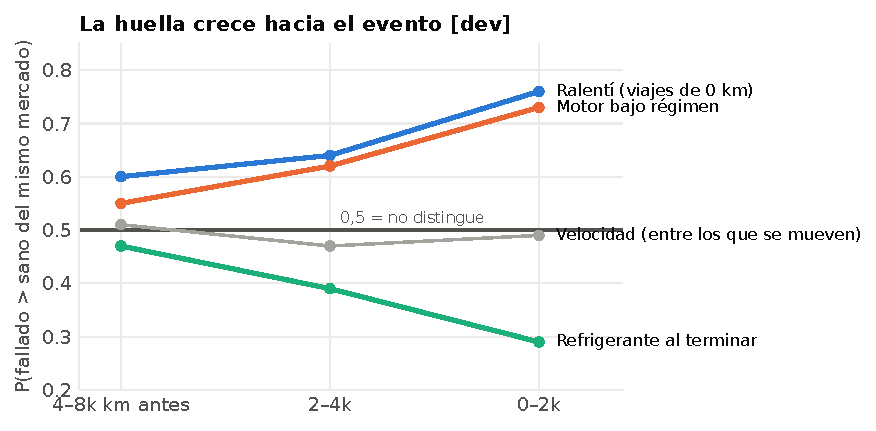
\includegraphics[width=0.9\textwidth]{figuras/perfil_evento.pdf}
\caption{Probabilidad de que un auto que va a fallar supere a un sano del mismo mercado y del mismo tramo de
odómetro, según la distancia al evento. Ralentí y bajo régimen crecen hacia el evento; el refrigerante
termina los viajes más frío. La velocidad no distingue dentro del mercado.}
\label{fig:perfil}
\fuente{\repo{docs/\allowbreak{}memoria/\allowbreak{}f9-eda-v2.md} §E (dev, 103–132 fallados por tramo); figura:
\repo{scripts/\allowbreak{}make\_report\_figures.py}.}
\end{figure}

\begin{itemize}
  \item \textbf{La huella crece hacia el evento} (figura~\ref{fig:perfil}). Lo que crece es estar detenido con
    el motor en marcha y no llegar a temperatura, no manejar distinto. Con la referencia corrida tres semanas
    la tendencia se sostiene. Lejos del evento (4.000–8.000 km, unos 3–5 meses antes) la señal es débil.
  \item \textbf{Se ve temprano.} Con las features de los primeros 60 días después de la venta, el ralentí
    ordena autos con AUC 0,636 dentro del mercado (125 fallados, 298 sanos). Es señal de \emph{qué auto},
    disponible desde el primer o segundo mes.
  \item \textbf{Algunas cosas van al revés de lo esperado}: los que fallan terminan los viajes con el filtro
    levemente \emph{menos} cargado (0,40–0,45) y regeneran algo menos por km (0,40–0,45). Por eso al
    conductor nunca se le nombra el estado del filtro (§\ref{sec:explicabilidad}).
  \item \textbf{La temperatura ambiente de los fallados es más baja} que la de los sanos de su mercado
    (0,37–0,45), también contra el mismo mes: no es estación sino lugar. Una parte del “bajo régimen” puede ser
    clima de la ciudad. Por eso la temperatura ambiente no entra al modelo.
\end{itemize}

\begin{figure}[H]
\centering
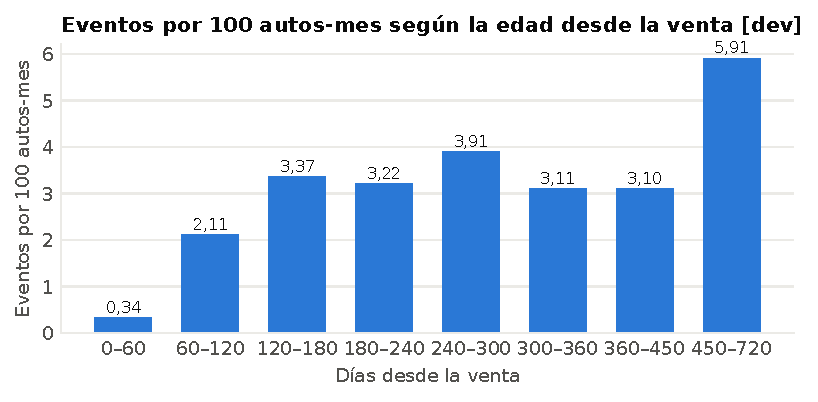
\includegraphics[width=0.9\textwidth]{figuras/riesgo_edad.pdf}
\caption{Riesgo por días desde la venta (Poisson con exposición, un registro por auto-día hasta el evento o el
fin de extracción). Sube hasta los \textasciitilde4 meses y entre los 4 y los 15 meses queda en
\textasciitilde3–4 eventos por 100 autos-mes.}
\label{fig:riesgo}
\fuente{\repo{docs/\allowbreak{}memoria/\allowbreak{}f9-eda-v2.md} §B (dev).}
\end{figure}

\textbf{El riesgo es de edad, no de kilómetros} (figura~\ref{fig:riesgo}). Ajustando por días desde la venta,
mercado y motor, el mes calendario no agrega nada (p = 0,16): no hay una ventana del registro. Lo que sí
agrega es la \emph{cohorte de venta}: los vendidos en el primer trimestre de 2025 fallan 2,1 veces más que los
del segundo a igual edad (p = 0,005). Es el mismo gradiente de producción del universo, y por eso las fechas
quedan fuera del modelo.

\begin{figure}[H]
\centering
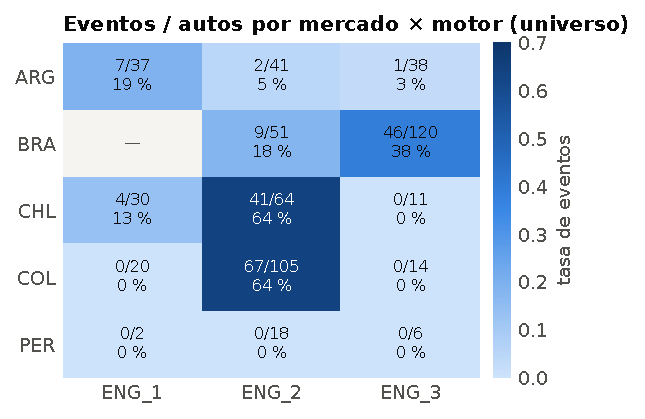
\includegraphics[width=0.62\textwidth]{figuras/celdas.pdf}
\caption{Eventos sobre autos por mercado × motor en el universo de 557. Tres celdas concentran casi todas
las fallas. Las tasas por mercado están cruzadas con cómo Ford armó la lista de fallados, así que no se leen
como física del mercado.}
\label{fig:celdas}
\fuente{\repo{docs/\allowbreak{}memoria/\allowbreak{}f9-universo-v2.md} §3.}
\end{figure}

\textbf{Dónde se concentra} (figura~\ref{fig:celdas}). En el universo, Colombia × ENG\_2 (67 de 105), Chile ×
ENG\_2 (41 de 64) y Brasil × ENG\_3 (46 de 120) concentran casi todas las fallas. Dentro de Brasil, ENG\_3 falla
2,5 veces más que ENG\_2 a igual edad, mientras que en Chile y Colombia ENG\_1 y ENG\_3 casi no fallan. Esto
define el piso más exigente del proyecto: saber mercado y motor, sin mirar un solo viaje, ya ordena muchísimo.
Qué parte de esa tasa es física (combustible, altura, motor) y qué parte es cómo se armó la lista no se puede
separar con estos datos: es la pregunta más importante para Ford.

\subsection{Consistencia y trazabilidad del pipeline}
\label{sec:trazabilidad}

\begin{itemize}
  \item \textbf{Las correcciones de los crudos se declaran, no se programan sueltas.} El loader
    (\repo{src/\allowbreak{}data/\allowbreak{}loader.py}) aplica por parte y por tabla lo que dice \repo{configs/\allowbreak{}data/\allowbreak{}raw\_sources.yaml}:
    renombres, corrimientos de origen, corte en el fin de extracción y formato de fechas. La entrega 1 se
    sigue leyendo con su propio YAML (\repo{raw\_sources\_v1.yaml}), bit a bit.
  \item \textbf{Un solo lugar por decisión.} El universo vive en \repo{src/\allowbreak{}data/\allowbreak{}usable.py}, los clones en
    \repo{configs/\allowbreak{}data/\allowbreak{}vehicle\_dedupe.yaml}, el split en \repo{src/\allowbreak{}eval/\allowbreak{}splits.py}. El recorte a desarrollo se
    hace por pertenencia explícita a la lista congelada, y el código falla si el panel trae un vehículo
    excluido (señal de que se construyó con el universo viejo).
  \item \textbf{Holdouts congelados y reproducibles.} El de la entrega 1 se reproduce bit a bit (huella
    \texttt{ba9aa4d290bc6610}); el de la v2 guarda además qué autos estaban del otro lado antes.
  \item \textbf{Contrato de datos por prefijo.} Toda columna que entra a un modelo se llama \texttt{feat\_} o
    \texttt{static\_}; lo que sirve para auditar se llama \texttt{aux\_} y el entrenamiento no lo puede ver.
    Agregar una feature es una línea de YAML.
  \item \textbf{Nada se hardcodea}: cada corrida es un YAML versionado en \repo{configs/\allowbreak{}}, y sus métricas y su
    configuración completa quedan en \repo{results/\allowbreak{}}. Los paneles y el holdout se publican como artefactos de
    Weights \& Biases, en un único proyecto compartido.
  \item \textbf{Chequeos automáticos} (\repo{scripts/\allowbreak{}check\_setup.py}, más de 200) que cubren el contrato, las
    trampas de formato y las reglas antileakage; se corren antes de cada merge.
  \item \textbf{Cada hallazgo tiene su evidencia y su comando} en \repo{docs/\allowbreak{}memoria/\allowbreak{}}, y cada decisión su fecha
    y su motivo en \repo{docs/\allowbreak{}memoria/\allowbreak{}decisiones.md}. Los comandos para reproducir este informe están en el
    Anexo~\ref{anx:repro}.
\end{itemize}
